\documentclass[12pt]{article}
\usepackage{amsmath}
\usepackage{graphicx}
\usepackage{multirow}
\begin{document}
\title{Computer Science M151B, Homework 6}
\date{May 14th, 2018}
\author{Michael Wu\\UID: 404751542}
\maketitle

\section*{Problem 1}

The average rotational latency will be
\[\frac{\frac{1}{2}\text{ rotations}}{5400\text{ RPM}\times \frac{1 \text{ minute}}{60 \text{ s}}}=0.00555\ldots \text{ s}\]
and because the data is located sequentially in memory, the additional overhead of reading the two additional sectors after the first is negligible.
Thus we can add the \(0.004 \text{ s}\) seek time to the rotational latency to obtain the total time to read the data, which is approximately
\[0.0096\text{ s}\]

\section*{Problem 2}

Transferring 64 bits of data from the I/O device to memory will take two bus transfers, as the CPU must perform a read and a write. Thus
the maximum possible bandwidth at which data can be transferred between the device and memory is
\[\frac{64 \text{ bits} \times \frac{1 \text{ byte}}{8 \text{ bits}}}{2\times 12 \text{ ns} \times \frac{1 \text{ s}}{10^9 \text{ ns}}}
=3.33333333 \times 10^8 \,\frac{\text{bytes}}{\text{s}}\]

\section*{Problem 3}

The total time it takes for a disk access is
\[0.0045 \text{ s}
+0.0003 \text{ s}
+\frac{\frac{1}{2}\text{ rotations}}{12000\text{ RPM}\times \frac{1 \text{ minute}}{60 \text{ s}}}
+\frac{4 \text{ KB}\times \frac{1\text{ MB}}{1000 \text{ KB}}}{80 \frac{\text{ MB}}{\text{s}}}
=0.00735 \text{ s}\]
and the processing time takes
\[\frac{2\times 10^7}{5\times 10^9 \text{ Hz}}=0.004 \text{ s}\]
Because there are two disk accesses and one processing step, the total time to process a block is
\[2\times 0.00735 \text{ s} + 0.004 \text{ s} = 0.0187 \text{ s}\]
and so the number of blocks processed per second is
\[\frac{1 \text{ block}}{0.0187 \text{ s}}=53.476 \,\frac{\text{blocks}}{\text{s}}\]

\section*{Problem 4}

\paragraph{a)}

Assuming that the process does nothing but poll while waiting for the device to send data, the polling will take
\[0.00002 \text{ s} \times 1.8 \times 10^9 \text{ Hz} = 36000 \text{ cycles}\]
and the processing will take an additional 1000 cycles. Since 1000 bytes need to be processed, the entire operation
takes 37 million cycles. I am assuming that the time spend waiting for the device to send data does not overlap with
the time spent receiving and processing the data.

\paragraph{b)}

Since 36000 cycles will be spent waiting for the device and 200 cycles are needed as overhead for handling interrupts,
this leaves 35800 cycles between each data read that can be used by another process. Since there will be 1000 bytes
read, this means that overall there are 35.8 million cycles available for use over the entire operation.

\section*{Problem 5}

\paragraph{a)}

No.

\paragraph{b)}

The forwarding unit only affects instructions after the ones currently in the pipeline. Since normal execution occurs up until
the \texttt{EX} stage of the instruction that generates the exception, all instructions prior to that instruction have the
correct data forwarded. The modified processor inserts bubbles into the pipeline so that these instructions complete before
starting the exception handler. So the forwarding unit does not need to change, as there are no data dependencies from the
last correct instruction executed and the start of the exception handler.

\section*{Problem 6}

\paragraph{a)}

I would simply add a new control signal from the control unit called \texttt{IllegalOp}, store it into the \texttt{ID/EX} register,
then wire that back to the control unit. This way exceptions are only handled during the \texttt{EX} stage, so conflicts between
exceptions from instructions which are in the pipeline at the same time do not occur. Then based on the \texttt{IllegalOp} signal,
the control unit can output the correct signals to flush the registers and change the program counter to the address of the exception
handler.

\pagebreak

\begin{figure}[!ht]
        \hspace*{-4cm}
        \begin{center}
                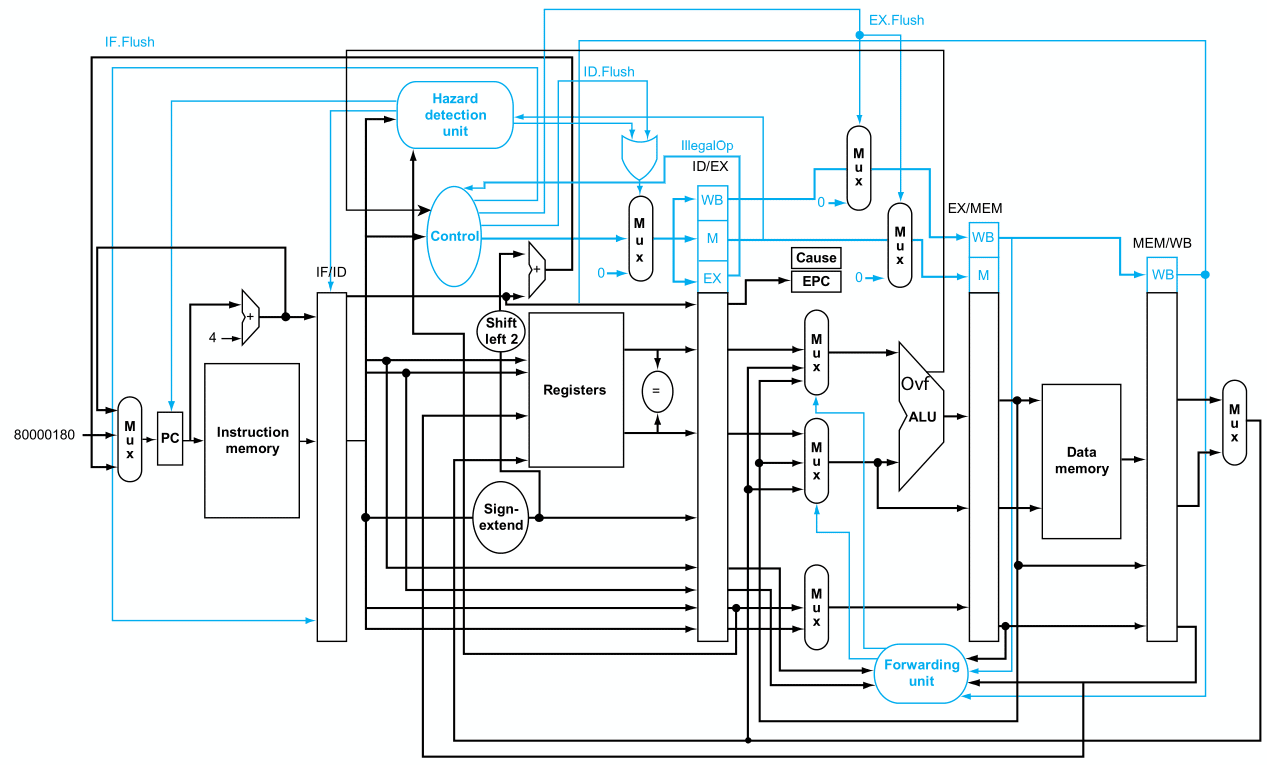
\includegraphics[width=5in]{problem6b.png}
        \end{center}
        \hspace*{-4cm}
\end{figure}

\paragraph{b)}

The modification to the datapath is shown in the figure above.

\paragraph{c)}

The signal \texttt{IllegalOp} will be added as shown above. It will be fed back into the control unit during the \texttt{EX} stage which will
eliminate problems with overflows and illegal instructions occuring at the same time. A combinational circuit that checks for all illegal opcodes
can implement this signal.

\paragraph{d)}

The control unit logic can be implement with the following table. I assume that \texttt{CauseSRC} will be 0 to indicate an overflow, and 1 to indicate an
illegal operation.

\begin{center}
        \hspace*{-4cm}
        \begin{tabular}{c|c|c|c|c|c|c}
                & Signals & Normal & Branch & IllegalID & Overflow & IllegalEX\\
                \hline
                \multirow{3}{*}{Inputs} & Overflow & 0 & 0 & 0 & 1 & x\\
                & IllegalOp & 0 & 0 & 0 & 0 & 1\\
                & Opcode & Legal, not 4 & 4 & Illegal & x & x\\
                \hline
                \multirow{8}{*}{Outputs} & IF.Flush & 0 & 1 & 0 & 1 & 1\\
                & ID.Flush & 0 & 0 & 0 & 1 & 1\\
                & EX.Flush & 0 & 0 & 0 & 1 & 1\\
                & IllegalOp & 0 & 0 & 1 & x & x\\
                & Orig. Signals & Orig. & Orig. & x & x & x\\
                & EPCWrite & 0 & 0 & 0 & 1 & 1\\
                & CauseWrite & 0 & 0 & 0 & 1 & 1\\
                & CauseSrc & x & x & x & 0 & 1
        \end{tabular}
        \hspace*{-4cm}
\end{center}

\end{document}